\chapter{Methodology}
\label{chap:methodology}

\section{Development of the simulation model}

\subsection{Specifications}
\label{sub:spec}

The aim of the model is to be able to simulate the production of a single power plant as well as to execute state or country-wide simulations. It should take entries from the OpenEnergy Database as input and be able to run solely on these inputs, i.e. to simulate the production knowing only the location and nominal power of the plants, without further information on their design (see sec. \ref{sub:hpp_reg}). 
The desired outputs for the model are electricity production time series per power plant or per area.


\subsection{Performance calculation}
\label{sub:perf_calc}

The electricity production of a power plant will be calculated using the characteristic equation of hydroelectricity (eq. \ref{eq_power_2} obtained page \pageref{eq_power_2}).

\begin{equation*}
 P = \rho_\mathrm{water} \cdot g \cdot \min(\dot{V}_\mathrm{n},\dot{V}-\dot{V}_\mathrm{rest}) \cdot (h_\mathrm{n} +W_\mathrm{n}-W) \cdot \eta_\mathrm{turbine} \cdot \eta_\mathrm{generator}\tag{\ref{eq_power_2} revisited}
\end{equation*}

In order to use this equation, the following parameters and values would be needed : 

\begin{itemize}
\itemsep0em
 \item Power plant parameters : 
 \begin{itemize}
  \item nominal water flow through the turbine ($\dot{V}_\mathrm{n}$)
  \item nominal head of water ($h_\mathrm{n}$)
  \item nominal water level ($W_\mathrm{n}$)
  \item efficiency curve of the turbine ($\eta_\mathrm{turbine}$) 
  \item efficiency curve of the generator ($\eta_\mathrm{generator}$)  
  \item residual water flow ($\dot{V}_\mathrm{rest}$)  
 \end{itemize}
 \item Input time series : 
 \begin{itemize}
  \item actual water flow through the turbine ($\dot{V}$)
  \item actual water level downstream from the turbine ($W$)
 \end{itemize}
\end{itemize}

However, if such precise data can be found for single power plants, it is not easily accessible at a state or country-wide level and not present in the OEDB or in the Marktstammdatenregister. 
Therefore, the model should be able to extrapolate missing data and to make some assumptions when optional input parameters are not provided. The only compulsory input parameter will be the broadly available nominal power of the turbine and subsection \ref{sub:assumptions} explains how other parameters can be assumed or extrapolated. \newline
In terms of time series, in addition to the water flow over the simulated period, the model will take as input the water flow over several years in order to extrapolate missing parameters.
The efficiencies of the generator and of the tubine will be calculated using respectively the values given in tables \ref{eta_gen} page \pageref{eta_gen} and \ref{eff_param} page \pageref{eff_param}.

\subsection{Simplifications and extrapolation of missing data}
\label{sub:assumptions}

A specification of the model, as explained in subsection \ref{sub:spec}, is to be able to run the simulation with limited information about the power plant, namely the nominal power and the coordinates. To do so, some simplifications will be used and other necessary information (nominal head, nominal inflow, and type of turbine) will be extrapolated from the hydrological history of the location, following the steps of the design process for a run-of-the-river plant.
\subsubsection{Approximation of the head by the nominal head}

The equation \ref{eq_head} given on page \pageref{eq_head} gives the relation between the head and the water level. However, it is not possible to know the water level directly after a power plant without having a gauge station exactly there. Section \ref{sec:meas_runoff} shows that measured data for water level is widely available throughout Germany, however the gauge stations are not bound to power plants and the water level directly downstream from a plant cannot be approximated with a value measured somewhere else on the river, because it depends on the shape of the river bed : figures \ref{mosel_WQ} based on measurement data for three stations on the Mosel from the Deutsches Gewässerkundliches Jahrbuch show linear correlations with different slopes between water level and water flow, and figure \ref{W_mosel} shows that the water level does not depend on the distance to the river mouth (see appendix \ref{app:boxplot} on how to read the graph). \newline
This strong variability of water level from a place to another would biase the results if the equation \ref{eq_head} (p.\pageref{eq_head}) was used with measured water level as input. Moreover, the modeled river data will not include information on the water level. For these reasons, the model will approximate the head of water $h$ with the nominal head $h_\mathrm{n}$.

\begin{figure}[H]
\centering
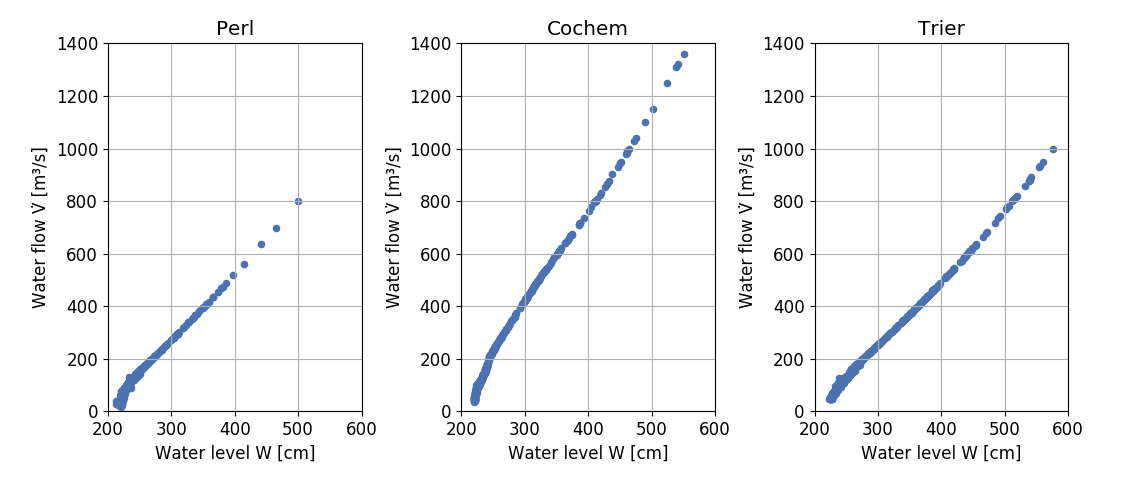
\includegraphics[width=15cm]{mosel_WQ.png}
\caption[Linear correlation between water level and  water flow for three places on the Mosel]{Linear correlation between water level and water flow for three places on the Mosel, data from \cite{dgj}, year 2014}
\label{mosel_WQ}
\end{figure}


\begin{figure}[H]
\centering
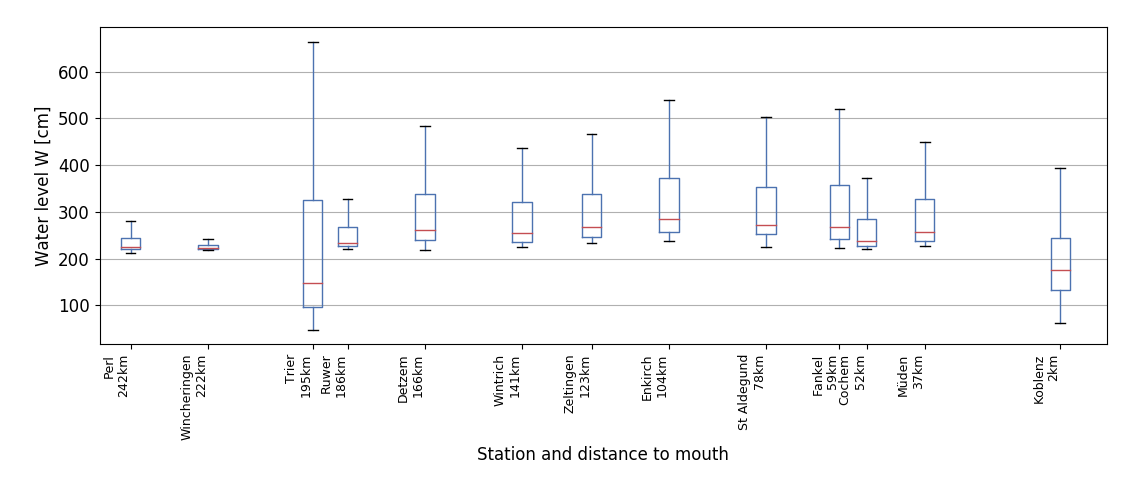
\includegraphics[width=15cm]{W_mosel.png}
\caption[Distribution of water level at gauges on the Mosel]{Distribution of water level at gauges on the Mosel, data from \cite{dgj}, year 2014}
\label{W_mosel}
\end{figure}

\subsubsection{Calculation of the residual water flow}
\label{sub:extrapol_dV_rest}

The residual water flow \.V\textsubscript{rest} is regulated by law, and therefore depends on the country, or on the federal state in Germany. Giesecke gives several ways of defining the residual water quantity and shows that they give slightly differents values \cite{gies_qrest}. In this work, a formula-based approach was used to calculate the residual water (see tab. \ref{res_wat}), where \.{V}\textsubscript{347} is the water flow reached or exceeded 347 days a year, averaged over 10 years. 
\begin{table}
 \centering
 \caption[Residual water quantity depending on the river]{Residual water quantity depending on the river \cite{gies_qrest}}
 \label{res_wat}
 \begin{tabular}{|l|c|}
  \hline
  \multicolumn{1}{|c|}{\.{V}\textsubscript{347} [\unit{l\textperiodcentered s\textsuperscript{-1}}]}& \.{V}\textsubscript{rest} [\unit{l\textperiodcentered s\textsuperscript{-1}}]\\
  \hline
  Up to 60&50\\
  And for each further 10 & 8 more\\
  \hline
  For 160&130\\
  And for each further 10 & 4.4 more\\
  \hline
  For 500&280\\
  And for each further 100 & 31 more\\  
  \hline
  For 2500&900\\
  And for each further 100 & 21.3 more\\  
  \hline
  For 10000&2500\\
  And for each further 1000 & 150 more\\  
  \hline
  From 60000&10000\\
  \hline
 \end{tabular}
\end{table}

\subsubsection{Calculation of the nominal water flow}
\label{sub:extrapol_dV_n}

The nominal water flow is chosen so that the power plant works at full load a given number of days a year. The literature recommends that the nominal water flow should be reached 50 to 90 days a year for a system connected to the grid, or 250 days a year for an isolated operation (self-production) \cite{pacer}\cite{cetmef}. The value of 120 days (30\% of the year) can also be found \cite{cetmef}. The nominal water flow is obtained by analyzing the flow duration curve over as many years as possible. This work will use the value of 73 days a year (20\% of the year). However, this can lead to errors, as the real value is influenced by economical and human factors.

\subsubsection{Calculation of the nominal head}
\label{sub:extrapol_h_n}

Even though the potential head of water could be calculated from the altitude variations along the river, it would be difficult to assess what is technically and economically feasible, without precise information on the location. However, the nominal head can be easily calculated from the nominal water flow and the nominal power, using equation \ref{head_calc}. At this point of the process, the type of turbine is not known. However, figure \ref{efficiency_turb} page \pageref{efficiency_turb} shows that at full load, all types of turbines have an efficiency around 90\%.

\begin{equation}
\label{head_calc} 
 h = \frac{P_\mathrm{n}}{\rho_\mathrm{water} \cdot g \cdot \dot{V}_\mathrm{n} \cdot \eta_\mathrm{turbine,n} \cdot \eta_\mathrm{generator,n}}
\end{equation}

\subsubsection{Deduction of the turbine type}
Finally, the type of turbine is deduced from the nominal head and nominal water flow using a characteristic diagram (fig. \ref{charac_diag}). 

\begin{figure}[H]
\centering
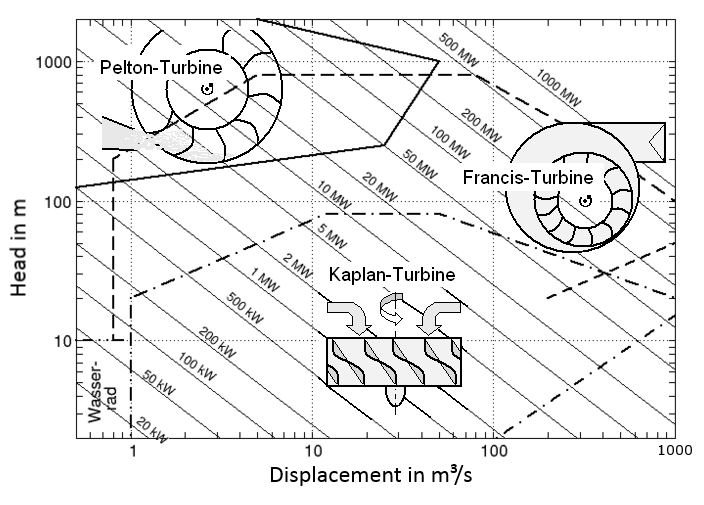
\includegraphics[width=12cm]{charac_diag_en.png}
\caption[Characteristic diagram for several types of water turbines]{Characteristic diagram for several types of water turbines \cite{wiki_WK}}
\label{charac_diag}
\end{figure}

\subsection{Necessary input data}
\label{sub:collec_data}

Considering the assumptions made in the previous subsection (sec. \ref{sub:assumptions}), the list of necessary data from subsection \ref{sub:perf_calc} becomes :
\begin{itemize}
 \item Water flow data (time series for the period to simulate)
 \item Geographical data (river courses)
 \item Properties of installed run-of-the-river power plants :
 \begin{itemize}
  \item Coordinates
  \item Installed capacity
  \item Nominal head or nominal inflow or history of water flows
  \item Type of turbine or characteristic diagram of turbines
 \end{itemize}
 \item Real production data for validation
\end{itemize}

This data has to be collected and pre-processed to serve as input for the model (see section \ref{sec:data_preproc}).

\section{Data preprocessing}
\label{sec:data_preproc}
The input data listed in subsection \ref{sub:collec_data} and obtained by the sources cited in subsection \ref{sec:simu_res} have to be preprocessed in order to be read by the model.

\subsection{Power plants register - OEDB}
\label{sub:pp_reg}

The OEDB register containing information about run-of-the-river power plants is the table ``ego{\_}dp{\_}res{\_}powerplant'' in the schema ``supply''. It is a register for renewable power plants, classified by technology through the column generation{\_}type (solar, wind, geothermal, run{\_}of{\_}river, gas, biomass). \newline 
The map of OEDB run-of-the-river power plants and German rivers shows that the localization of the plants is not always accurate (see fig. \ref{pp_river_dist}).
\begin{figure}[H]
\center
\framebox{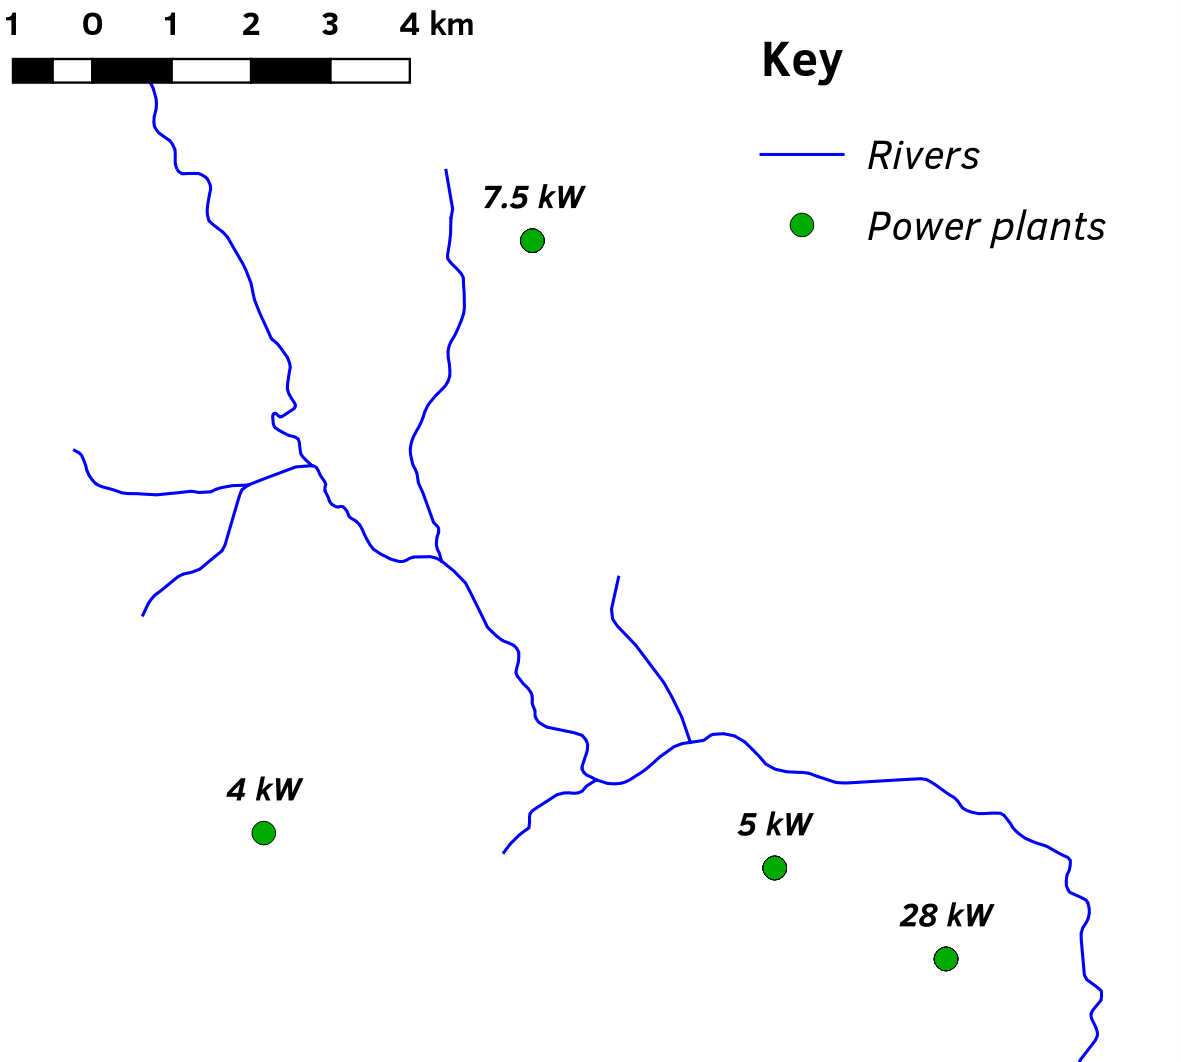
\includegraphics[width=10cm]{pp_river_dist.png}}
\caption{Inaccuracy of plant locations}
\label{pp_river_dist}
\end{figure}
The first step of data preprocessing is to assign a river to each plant and relocate that plant on the river. \newline
In the case of modeled runoff data (see sec. \ref{sec:mod_runoff}), this will ensure that the plant is in the same grid cell as the river, and in the case of measured runoff data (see sec. \ref{sec:meas_runoff}), this will allow the assignment of a gauge station from the same river to the plant.


\subsubsection*{River identification and relocation of power plants}

This is made with SQL queries. The register of all rivers in Germany was created from the Digital Landscape Model (DLM250) of the german Federal Agency for Cartography and Geodesy. This model describes the topographic features of the landscape in the vector format and is made available as open data \cite{dlm250}. \newline Two types of features were used : ``57003 AX{\_}Gewaesserstationierungsachse'' from the layer GEW03 give the main rivers and ``44004 AX{\_}Gewaesserachse'' from the layer GEW01 give the secondary rivers. \newline 
SQL queries on the river segments and power plants geometries enabled the assignment of a river to each plant. This process is described in figure \ref{river_id} and takes place as follow : 

\begin{figure}[H]
\begin{center}
  \subfigure[Power plants and river layers]{\framebox{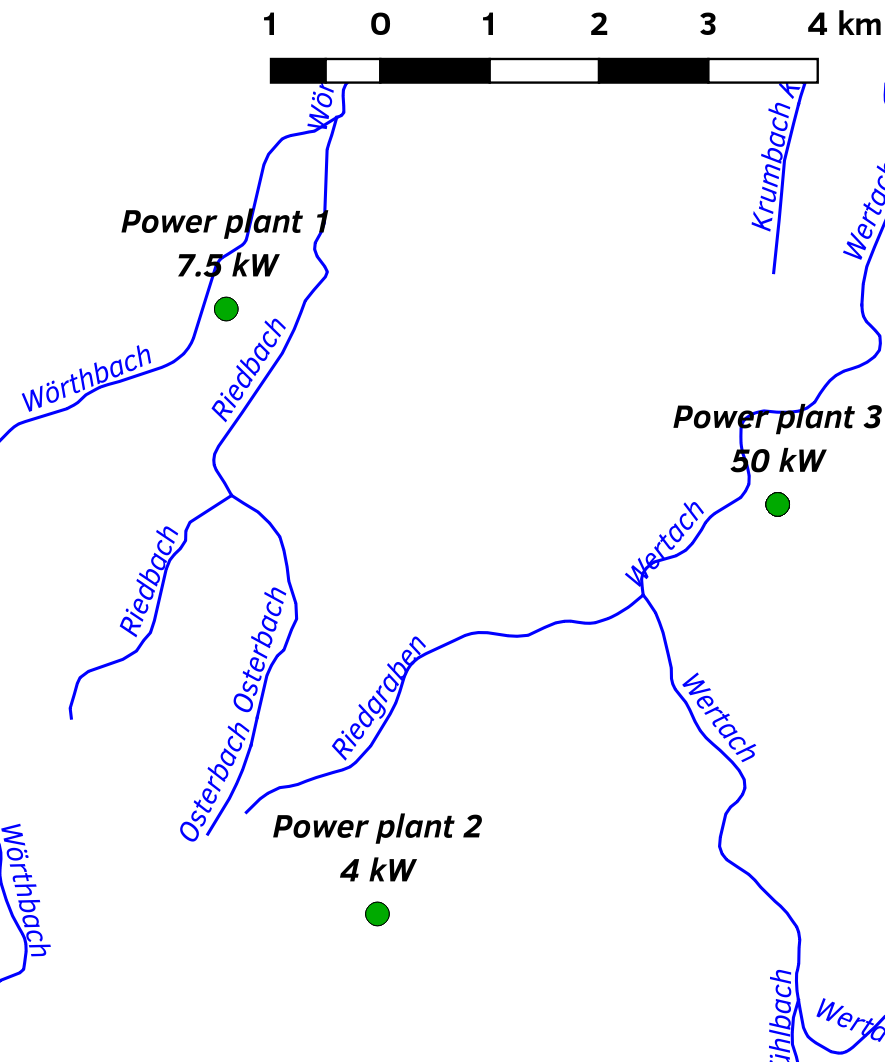
\includegraphics[width=5cm]{empty.png}}} \hspace{3cm}
  \subfigure[Rivers within {\unit[2]{km}} of plants]{\framebox{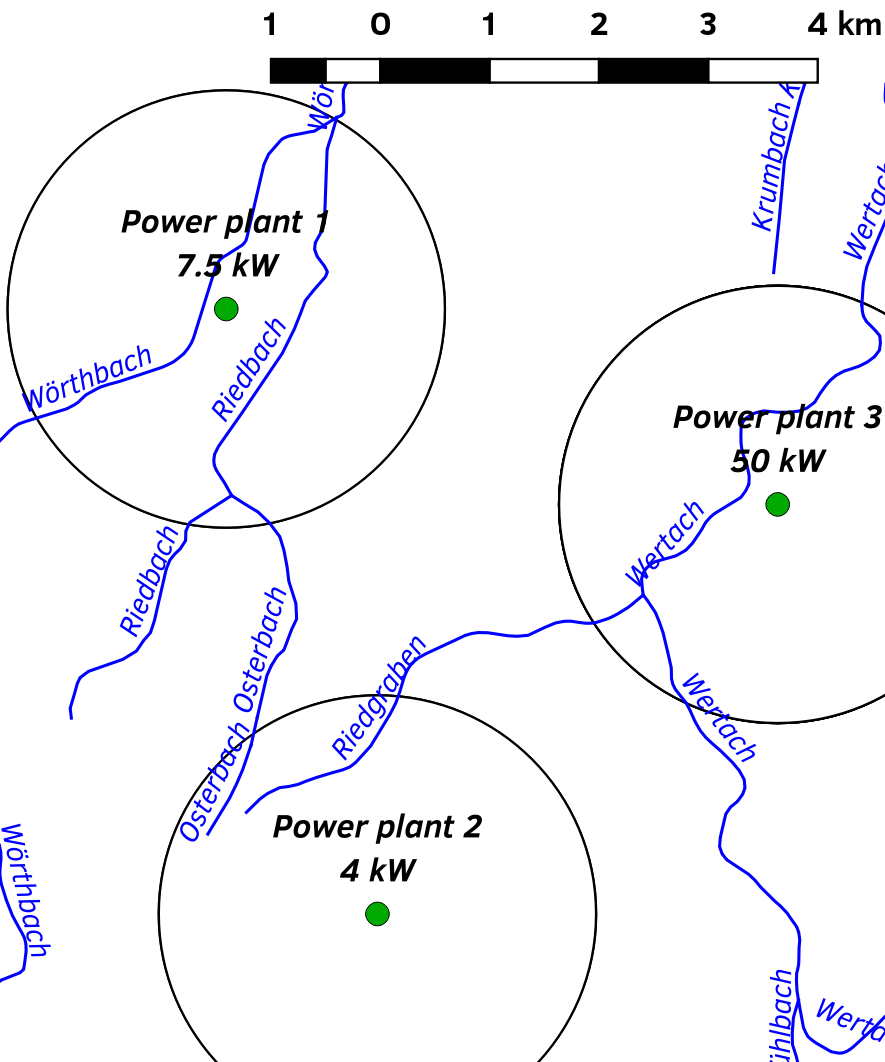
\includegraphics[width=5cm]{kreis.png}}} \\
  \subfigure[Shortest distance to each river]{\framebox{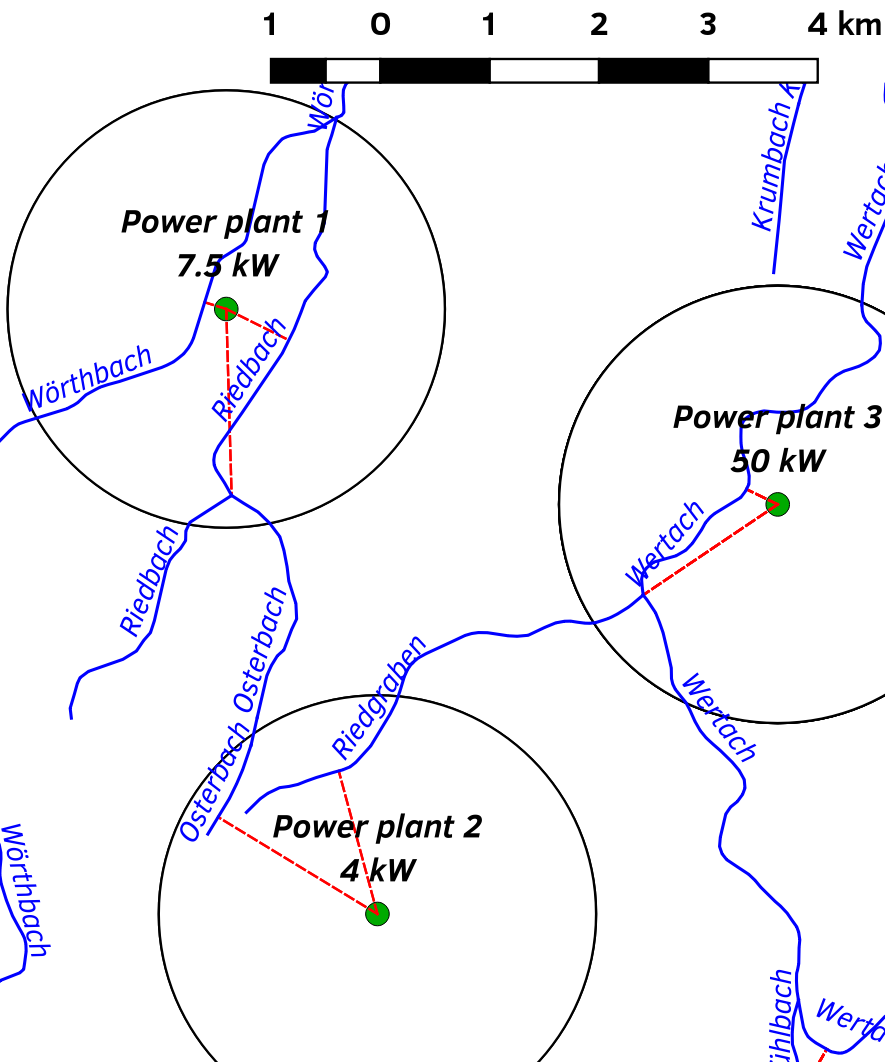
\includegraphics[width=5cm]{kreis_many_lines.png}}} \hspace{3cm}
  \subfigure[Keep the closest river]{\framebox{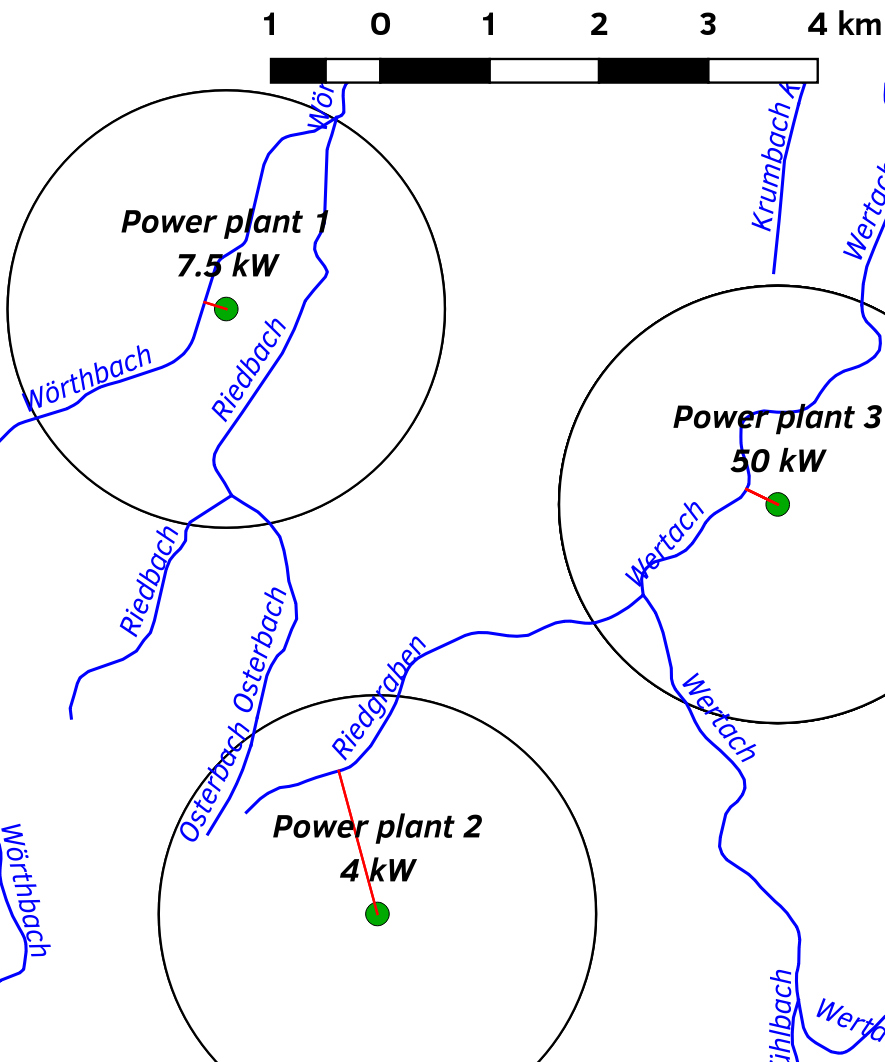
\includegraphics[width=5cm]{kreis_line.png}}} \\ 
  \subfigure[New positions of power plants]{\framebox{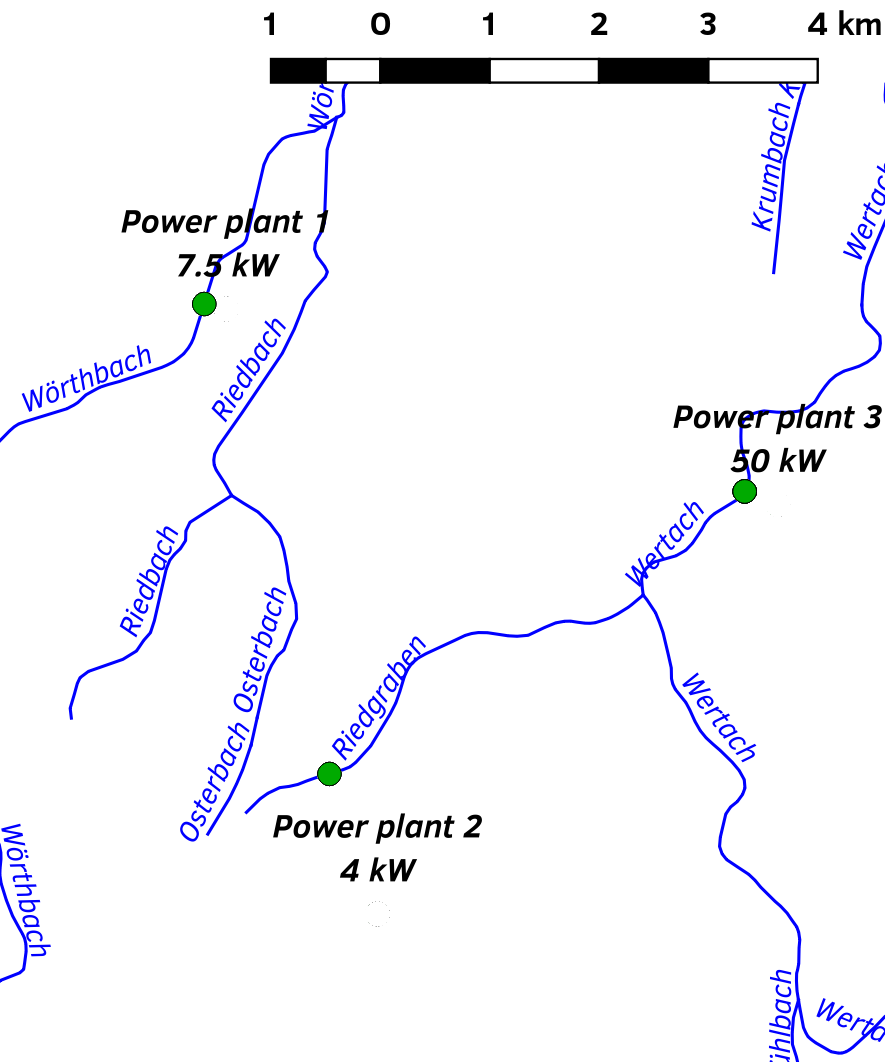
\includegraphics[width=5cm]{new.png}}}
\end{center}
\caption{River identification process}
\label{river_id}
\end{figure}

\begin{itemize}
 \item the function ``ST{\_}DWithin(power plant geometry, rivers geometry, 2000)'' locates all rivers in a \unit[2]{km} radius around each plant (fig. b)
 \item the function ``ST{\_}Distance(power plant geometry, rivers geometry)'' measures the  shortest distance to each river (fig. c)
 \item only the closest river is kept for each plant (fig. d)
 \item the plant is relocated by filling a new geometry column (dp{\_}geom) with the projection of the plant on the river using ``ST{\_}Endpoint(ST{\_}Shortestline(plant geometry, river geometry)''
\end{itemize}
The actual code is given in appendix \ref{app:sql_assign_river}.

\subsubsection*{Gauge assignment}
The next step is to assign each plant with a register of runoff time series. As discussed in sections \ref{sec:meas_runoff} and \ref{sec:mod_runoff} the runoff time series can either be measured or modeled. \newline
In the case of modeled data from WaterGap, runoff is given country wide with a resolution of 5 angular minutes vertically and horizontally (cells approximately \unit[9]{km} times \unit[6]{km}). The cells are located by their centers, and the assignment is made by finding the closest cell center for each plant. The process is similar to the river assignment process and the script is given in appendix \ref{app:sql_assign_watergap}. \newline
In the case of measured values, the stations are located on rivers across the country, with an inhomogeneous resolution. In this situation, runoff values from the same river, even further away from the plant, will be more accurate than those from a nearby tributary. The assignment process first looks for stations on the same river as the power plant, before looking for the next nearby station (script in appendix \ref{app:sql_assign_gauge}). Furthermore, only stations for which runoff data was available were considered (see sec. \ref{sec:runoff_data})

\subsection{Runoff data}
\label{sec:runoff_data}

Each type of runoff data (measured and modeled) is stored in the database with the following structure : a table listing the gauge stations or raster cells and their geometries (see tab. \ref{db_struct} left), and a table storing a runoff time series per year for each station (see tab. \ref{db_struct} right). In the database, runoffs are stored in \unit{m\textsuperscript{3}\textperiodcentered s\textsuperscript{-1}} with the letter 'Q' and water levels in \unit{cm} with the letter 'W'.

\begin{table}[H]
\footnotesize
  \centering
  \caption{Database structure for storing runoff time series}
  \label{db_struct}
  \begin{tabular}{|l|l|l|l|ll|l|l|l|l|l|l}
  \cline{1-5}\cline{7-12}
  id & geom &station & water & ...&& id & station & type & year & time series & ...\\
  \cline{1-5}\cline{7-12}
  1&geom1&name1&river1&...&&1&name1&Q&year1&\{q1,q2,q3...\}&...\\\cline{1-5}\cline{7-12}
  2&geom2&name2&river1&...&&2&name1&W&year1&\{w1,w2,w3...\}&...\\\cline{1-5}\cline{7-12}
  3&geom3&name3&river2&...&&3&name1&Q&year2&\{q1,q2,q3...\}&...\\\cline{1-5}\cline{7-12}
  4&geom4&name4&river3&...&&4&name1&W&year2&\{w1,w2,w3...\}&...\\\cline{1-5}\cline{7-12}
  5&geom5&name5&river3&...&&5&name2&Q&year1&\{q1,q2,q3...\}&...\\\cline{1-5}\cline{7-12}
  6&geom6&name6&river3&...&&6&name2&W&year1&\{w1,w2,w3...\}&...\\\cline{1-5}\cline{7-12}
  ...&...&...&...&...&&...&...&...&...&...&...\\
  \end{tabular}
\end{table}


\section{Simulation and evaluation of results}

\label{sec:simu_res}

In order to validate the model, the simulation results have to be compared to real data. This concerns the part of the model extrapolating plant parameters (sec. \ref{sub:assumptions}) as well as the calculation of production itself (sec. \ref{sub:perf_calc}). \newline
The model will be evaluated through simulations on :
\begin{itemize}
 \item A single power plant whose characteristics are known (nominal water flow, head, turbine type) with precise runoff data (hourly measures from a gauge within \unit[2]{km} of the plant). Objective : evaluating the quality of the production calculation.
 \item Power plants whose characteristics are known, simulated as entries from the OEDB, i.e. only with the nominal power. Objective : evaluating the extrapolation processes presented in subsection \ref{sub:assumptions}.
 \item A state-wide simulation based on the OpenEnergy Database. Objective : evaluating the quality of the whole process (preprocessing and simulation).
\end{itemize}

\subsection{Simulation of a single power plant}
\label{sub:metho_single}
The simulation will be conducted on a power plant whose parameters are known, giving a many inputs as possible. The Hydroraon power plant in the french Vosges department and operated by the company Ercisol was chosen for this simulation. Ercisol operates 4 run-of-the-river power plants in France and publishes the monthly productions on their website \cite{ercisol}. The power plant ``Hydroraon'' was chosen due to its proximity with a gauge station measuring water flow. The measured time series are made available on the ``Banque Hydro'' \cite{eaufrance}. This database is run by the SCHAPI (Service Central d'Hydrométéorologie et d'Appui à la Prévision des Inondations), a section of the french Ministry of Ecology, Sustainable Development and Energy, and gathers data from around 5000 gauge stations. \newline
The power plant has the following parameters :
\begin{itemize}
 \item P\textsubscript{n} \tabto{4cm}: \unit[400]{kW}
 \item Q\textsubscript{n} \tabto{4cm}: \unit[12]{m\textsuperscript{3}\textperiodcentered s\textsuperscript{-1}}
 \item H\textsubscript{n} \tabto{4cm}: \unit[4.23]{m}
 \item Number of turbines \tabto{4cm}: 1
 \item Type of turbine \tabto{4cm}: Kaplan
 \item River \tabto{4cm}: Meurthe
 \item Place \tabto{4cm}: Papeterie des Châtelles, Raon l'Étape
\end{itemize}

XX add period of time over which simu was made

\subsection{Extrapolation of missing plant parameters}

This process will be run on power plants whose characteristics (nominal head, nominal water flow, turbine types) are known, and for which measured values of water flow are available. \newline
The power plants of the Mosel were investigated because their characteristics are publicly available \cite{mosel} and the water flow is measured in three stations located in Cochem, Trier and Perl and run by the Wasserstraßen- und Schifffahrtsverwaltung des Bundes (WSV). The time series were made available by the Bundesanstalt für Gewässerkunde (BfG) and contain daily values over following timespans :
\begin{itemize}
 \item Cochem \tabto{2cm}: 1901 to 2016
 \item Perl \tabto{2cm}: 1975 to 2016
 \item Trier \tabto{2cm}: 1931 to 2016 except 1963 and 1964
\end{itemize}
XXX More plants : Raon, Kyll, ..., write this when the simu is done
XXX More details. Modeled data as well ?

\subsection{State-wide simulations} 
\label{sub:metho_sw}
The state wide simulations take the OEDB as power plant register. The simulated production is compared with the yearly production given by the AEE and presented in section \ref{sub:prod_data}. This section showed important discrepancies in installed capacity between the AEE data and the OEDB data. In order to minimize the impact of these discrepancies, the simulation will be run for Thuringe : among the three states for which the AEE data and the OEDB are consistent, this is the state with the biggest installed capacity, and it has no reservoir power plants listed in the OEDB. \newline
A simulation will be run with daily measured data from the Global Runoff Data Center (GRDC, Koblenz, Germany) and the Federal Waterways and Shipping Administration, provided by the Bundesanstalt für Gewässerkunde. Table \ref{quelle_runoff_th} lists the gauge stations and the timespans over which data was made available. The stations of Zoellnitz and Kaulsdorf-Eichicht were not used in this study because they do not have available data for the last decade.
\begin{table}
\footnotesize
 \centering
 \caption{Gauge stations in Thuringe}
 \label{quelle_runoff_th}
 \begin{tabular}{|l|l|l|l|}
  \hline
  \textbf{Station}&\textbf{River}&\textbf{Timespan}&\textbf{Source}\\
  \hline
  Eisenach-Petersberg&Hoersel&1940-2008&GRDC\\
  Dorndorf 2&Felda&1936-2008&GRDC\\
  Mittelschmalkalden&Schmalkalde&1956-2008&GRDC\\
  Ellingshausen&Hasel&1936-2011&GRDC\\
  Rappelsdorf&Schleuse&1951-2012&GRDC\\
  Arenshausen&Leine&1960-2011&GRDC\\
  Meiningen&Werra&1919-2012&GRDC\\
  Wasserthaleben&Helbe&1962-2011&GRDC\\
  Zoellnitz&Rode&1948-2003&GRDC\\
  Rudolstadt&Saale&1946-2008&GRDC\\
  Sundhausen&Helme&2005-2008&GRDC\\
  Nordhausen&Zorge&1954-2013&GRDC\\
  Niedertrebba&Ilm&1923-2013&GRDC\\
  Freienorla&Orla&1928-2010&GRDC\\
  Kaulsdorf-Eichicht&Loquitz&1923-2002&GRDC\\
  Moeschlitz&Wisenta&1925-2010&GRDC\\
  Weida&Weida&1961-2008&GRDC\\
  Goessnitz&Pleisse&1993-2008&GRDC\\
  Allendorf&Werra&1942-2016&BfG\\
  Heldra&Werra&1951-2016&BfG\\
  \hline
 \end{tabular}
\end{table}

Another simulation will be run with modeled runoff from the WaterGap software. XXX Add more details : number of cells in TH, timespan... 
